% based on:
%   apssamp.tex
% file that comes with Revtex.
%

\documentclass[letterpaper,twocolumn,amsmath,amssymb,prl,nolongbibliography,url,reprint]{revtex4-2}
%\documentclass[preprint,showpacs,preprintnumbers,amsmath,amssymb]{revtex4}

% Some other (several out of many) possibilities
%\documentclass[preprint,aps]{revtex4}
%\documentclass[preprint,aps,draft]{revtex4}
%\documentclass[prb]{revtex4}% Physical Review B

\usepackage{graphicx}% Include figure files
\usepackage{dcolumn}% Align table columns on decimal point
\usepackage{bm}% bold math
\usepackage{amsmath}

%\usepackage{url}
%\bibliographystyle{aipnum4-1}



\DeclareGraphicsExtensions{.eps,.EPS}

%\nofiles

\begin{document}

\preprint{}

\title{How to Win a Mapper Tournament (By Making Your Video Longer)}

%\title{AC Stark shift induced resonant electric dipole-dipole
%interactions between cold Rydberg atoms}%

\author{Noah Attamanchuk}
\email{nrattama@uwaterloo.ca}
\affiliation{%
Department of Physics and Astronomy \\
University of Waterloo, Waterloo, Ontario, N2L 3G1, Canada
}%

\date{\today}% It is always \today, today,
             %  but any date may be explicitly specified

\begin{abstract}
\textbf{\emph{The purpose of this report is to determine the length for a "Mapping" video that will most likely win a "Mapper Tournament".}}
We will analyze every Mapper Tournament hosted by the Mapping Community, where applicable, and break down the video lengths of each winner into 8 categories. We will then analyze these categories and determine which is the most likely to win. In addition, we will also determine the probability of winning a Mapper Tournament with minimal effort. In this case, that would be with a video of the shortest category.
\end{abstract}

\maketitle


Mapping is a YouTube genre defined by personifying countries on a digital map, to create and form a narrative around. The Mapping Community is a group of Mappers that specialize in creating these videos. Over the years, many competitions have been created around creating and producing these videos, the most popular of which being Mapper Tournament. 

Mapper Tournament, in it's more modern form, consists of a series of rounds where Mappers submit their projects to be graded by a series of judges. Once judges are finished, their results are released, and a few of the lowest scoring individuals are eliminated. This cycle is repeated consistently until there are only 4-6 competitors left, which compete in a final round. Whichever video wins the final round is crowned as the victor. 

The judging itself consists of ranking an aspect of the video from 1 to 10. This repeated across a series of judges, until the final scores are added up as sums. The rounds for this tournament all follow this procedure, so it is possible for there to be a "winner" in every round. 

As with any competition, we want to be able to make cuts in terms of how much work needs to be done in order to come out with a winning result. Ideally, we can determine if this can be done with the length of submitted Mapping videos. The longer our video is, the more time is needed need to commit to it. If it is possible to minimize this process, we should see how likely it is to do so.

During the lifespan of the Mapping Community, due to its nature as a genre, the community has insinuated that the length of videos has gotten longer. There is also a stigmatization that longer videos are "better" from a narrative and quality standpoint. We can potentially observe this stigmatization through the results we obtain, as all of the judges in and of themselves are community members. 

\textbf{\emph{How will we observe this, and determine our probabilities?}}

First of all, we will need to collect and define some values for video lengths. The Mapping Community has luckily archived a majority of its grading sheet for public viewing, so we can obtain these, refer to the videos that are linked with the results, and collect our video lengths. 

While we can do this for a majority of videos, there are two main problems with collecting data in this manner. First, some of the earlier Mapper Tournaments are from 2017-2018, where the videos have long since been purged off the website, making them lost media. Whenever we are unable to access a video length, it will be listed as \textbf{N/A}. Second, the format for these Mapper Tournaments have changed over the years. The early versions of the competition formatted their rounds into brackets, only merging competitors together in the qualifying and final round. We will therefore only look at those two rounds for the earlier Tournaments, marking the rest as \textbf{N/A}. For the sake of simplicity, and to correspond nicely with the number of competitors in a vast majority of final rounds, we will be looking at the top 5 scoring videos for each round.

Once all of our data is collected, we can categorize our data based on length. For this task specifically, we will break down the data into 8 separate quantiles. Since we are only analyzing the winners out of each top 5 ranking, we can get away with using evenly distributed quantiles for our data. We can then re-organize our previous data to fit our 8 quantiles, and then count up each winner from all of the rounds. We can showcase the number of wins each category has, and determine which length of video is preferable. We can then determine our probabilities by comparing the amount of wins with a specific video length to the total number of wins. 

We can also determine probabilities through multiple attempts by the Bionomial Distribution, which can be defined as:

\begin{equation}
f_{n,p}(r) = \binom{n}{r} p^r (1-p)^{n-r}
\end{equation}

Where r is is number of times a competitor has won a Mapper Tournament round, n is the number of attempts a competitor has taken, and p is the probability defined by our times and results. 

One last important point to consider is that these Tournaments have been taking place since 2015, and the types of Mapping videos being created have evolved since then. This is reflected in the level of grading for these Tournaments. To take this into account, there will be two versions of data analyzed. One that focuses on the entire datapool (From Mapper Tournament 5 to 27) and one focusing on the 10 most recent Mapping Tournaments (From 18 to 27).

\textbf{\emph{What does the data look like?}}

After analyzing all of the archived spreadsheets, we were able to determine 377 viable video lengths out of the top 5 competitors for each round. Their video's lengths are recorded in Figure 1 to the right of this paragraph.

We already notice an interesting trend with this data. We can see that earlier tournaments overall had shorter videos, compared to later on. Most videos in early MT (Abbreviation for Mapper Tournament) were between 1 to 10 minutes long. Compare this to MT23 and 24, where there are three 1 hour long videos out of 8 winners. This already indicates the stigma of needing to create longer videos over the course of the Tournament's lifespan.

We can now organize our data from shortest to longest, and determine quantiles by dividing our data into 8 increments, and determining where those increments end. When we determine that, we end up with the increments of time shown in Figure 2. We notice that despite the trend for longer and longer videos overtime, the quantiles we obtain are very balanced across a variety of times. A vast majority of videos seem to be less than 20 minutes long, with at least 1/8th being between 8 and 10 minutes in length. 

\begin{figure}
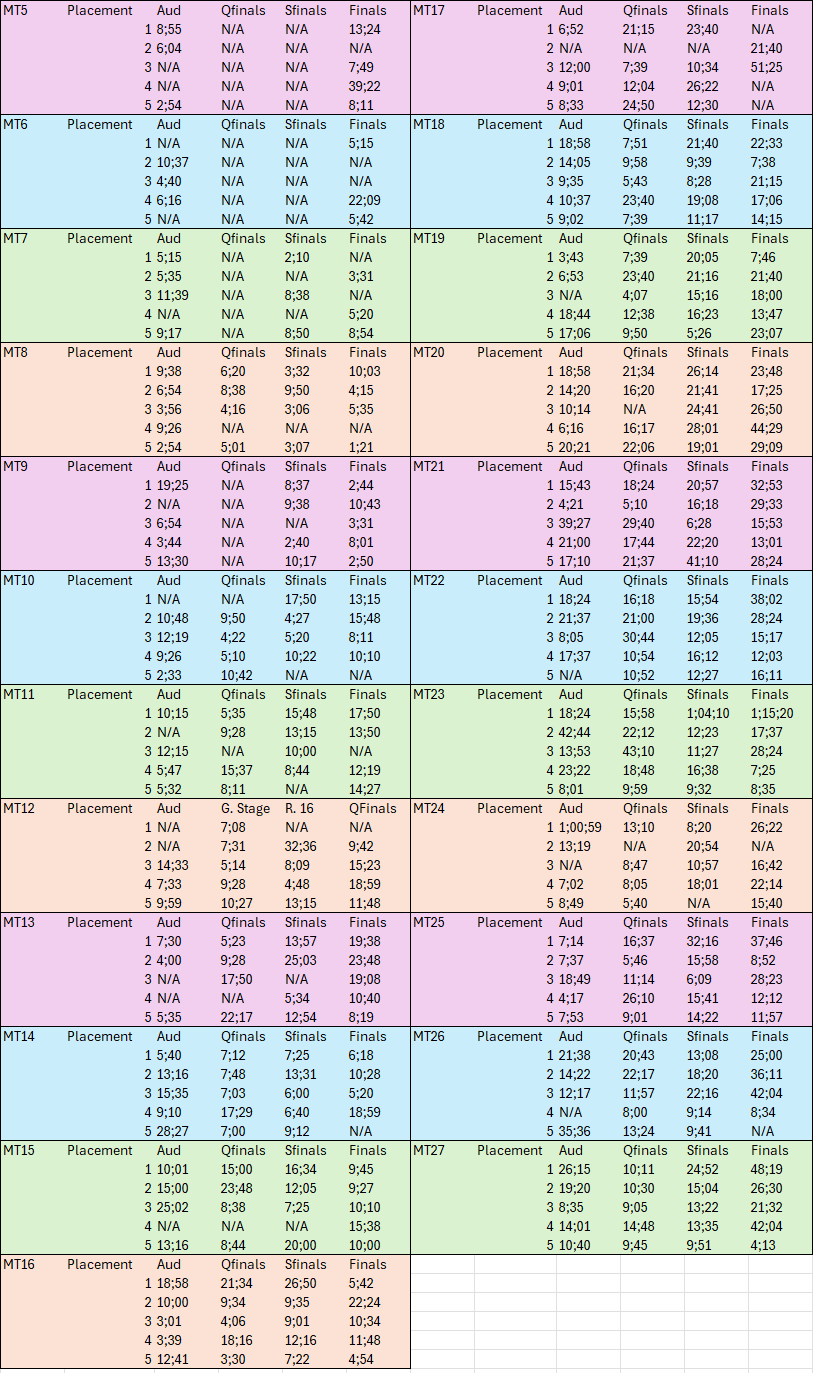
\includegraphics[width=1\linewidth]{Earlydata.png}
\caption{\label{fg:ret}
The length of all top 5 contending videos from Mapper Tournament 5 to Mapper Tournament 27. This information was taken directly from the Mapper Tournament spreadsheets.}
\end{figure}

We can than go back to Figure 1 and sub in our expressions for categories, defined in Figure 2, and apply them. With this (Figure 3), we obtain an updated table of data, which we can analyze and extract the winning video lengths from. Once we extract these values, we obtain our distribution.





\begin{figure}
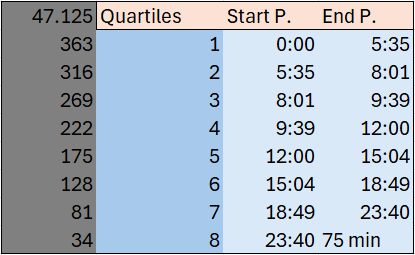
\includegraphics[width=1\linewidth]{quartiles.png}
\caption{\label{fg:ret} The quantiles used for this analysis. The grey values were used to find the in between points defining quantiles.
}
\end{figure}

\begin{figure}
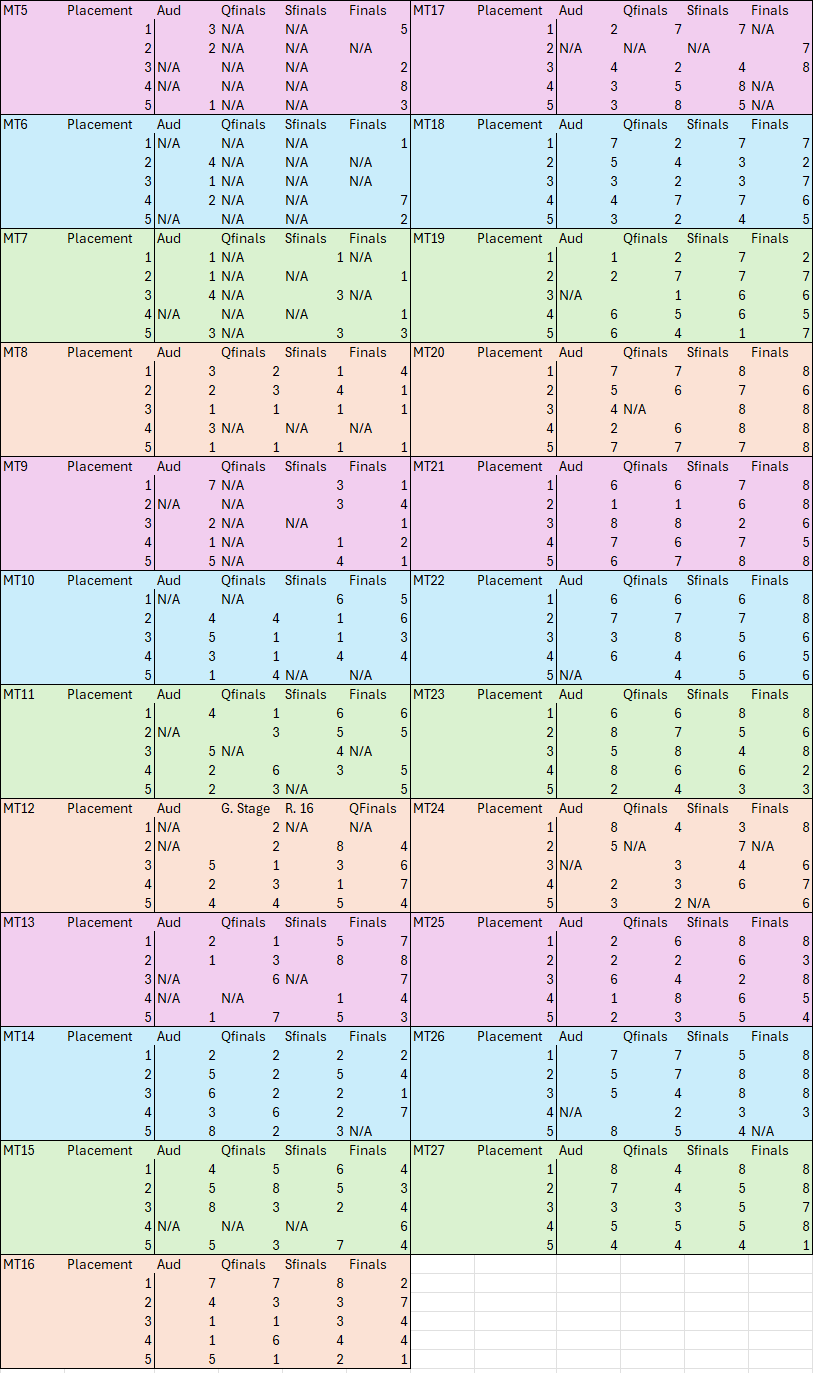
\includegraphics[width=1\linewidth]{Finaldata.png}
\caption{\label{fg:ret}
Our data from Figure 1, configured to the quartile/categories defined in Figure 2.}
\end{figure}

For the total amount of MT's, we can see that there are two distributions (Figure 4). One for videos around 5-8 minutes, and one for videos 18 minutes and longer. Our comments regarding increasing video length appear to be true, and grow even more apparent when we focus only on the last 10 MT's. Out of the original total value of 78 video lengths, 38 were removed by cutting out MT5 to MT17. The result of this, shown in Figure 5, is a massive decline in the original left disribution, and all categories from 0-15 minutes. Meanwhile, categories that consist of longer times hardly lose anything.

The result of this gives us an interesting perspective. As narrative Mapping evolves, it is assumed that videos should become longer to fit the growing complexity of those narratives. We can outright see this general qualitative opinion from a quantitative perspective, and we can see that opinion change overtime from Figure 4 to 5. With the data organized here, it can very easily be said that it is much easier to win a Mapper Tournament with a video over 20 minutes long. But by how much?

\textbf{\emph{How likely is it to win with a 5 minute video in a modern Mapper Tournament?}}

\begin{figure}
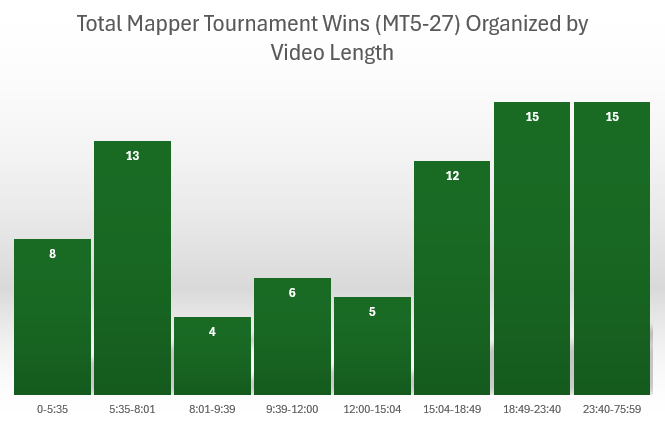
\includegraphics[width=1\linewidth]{fiveto27.png}
\caption{
\label{fg:acret} The total Mapper Tournament winning videos by video length, from MT5 to MT27.
}
\end{figure}

\begin{figure}
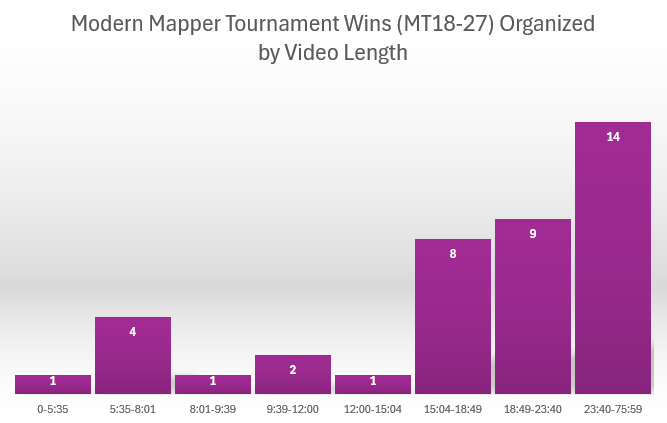
\includegraphics[width=1\linewidth]{eighteento27.png}
\caption{
\label{fg:acret} The modern Mapper Tournament winning videos by video length, from MT18 to MT27.
}
\end{figure}

In order to determine individual probabilities, we can just divide the number of wins in a specific time category (determined from our quantiles) by the total number of winning videos. This can be from either our total MT or modern MT data pool. 

With our total of 78 datapoints, we can determine our probabilities from our total number of wins. The shortest video category offers a 10.2\% chance of winning (8 divided by 78). The category from 5-8 minutes offers a 16\% chance of winning, and any video either between 18 to 23 minutes, or longer than 23 minutes has nearly a 20\% chance (19.2\%).

However, this is factoring in MT's from over 7-8 years ago, where our long video trend was not as apparent. If we want to have a good chance at winning, we should look at data that applies more to modern standards, that being Figure 5. Using the same method, and using the new total number of datapoints (40), we can determine the odds of winning with a video 23 minutes or longer to be a staggering 35\%. If we were to add the longest three categories and their probabilities, we obtain that producing a mapping video 15 minutes or longer gives a 77.5\% chance of winning. Our 0-5 minute category, meanwhile, offers a mere 2.5\% chance of victory.

However, our odds would become better if we were given more attempts. Using the bionomial distribution, we can determine the odds become 4.8\% after 2 attempts, and then 11.3\% after 5 attempts. As you can notice from our data in Figures 1 and 3, Mapper Tournaments tend to have 4 rounds in total. If we were to win just the final one, assuming we aren't eliminated in any of the previous rounds, we determine the odds of winning a Mapper Tournament with the shortest category of time:

\begin{equation}
f_{4,\frac{1}{40}}(r) = \binom{4}{1} (\frac{1}{40}) (\frac{39}{40})^3 = 9.2\%
\end{equation}

\textbf{\emph{Methods of improving this for the future, and discrepancies.}}

This analysis can be improved on by factoring in more placements, in order to gain potentially more accurate quantiles for our probabilities. It can also be improved through more data. Mapper Tournaments currently happen around 3 times a year, so obtaining more data eventually should not be difficult. It would be interesting to see if any patterns change, similar to what we saw between shorter and longer videos in our analysis. 

Overall, I am quite satisfied with the way the data was collected and analyzed, with the only notable error being present in our N/A values, which cannot be obtained anyway.

\textbf{\emph{To Conclude.}}

We determined that producing longer form Mapping videos is more likely to win you a Mapper Tournament through analysis of the past 10 MT's. If you want to put as little effort as possible time-wise, then any competitor would have a 9.2\% chance of winning any future MT, assuming they are able to make it through every round.

I would like to thank prominent community member "Sabyrcus" with offering the Mapper Tournament spreadsheets, as well as clarifying any mishaps or mistakes with the information presented in this work. 

\end{document}